%link do tworzenia tabeli https://tablesgenerator.com/
\documentclass{article}  %typ dokumentu
\usepackage[utf8]{inputenc} %rodzaj czcionki
\usepackage{geometry} %poprawienie marginesów
\usepackage{polski} %polskie znaki
\usepackage{multirow} %tabela
\usepackage{graphicx} %tabela
\usepackage{float} %tabela
\usepackage{diagbox} % 2 dane w jednym prostokącie
\usepackage{amsmath} % Matma
%\usepackage{blindtext} %
%\usepackage{enumitem}
\usepackage{tikz} %rysowanie

\usetikzlibrary{arrows}
\graphicspath{{pictures/}}
\geometry{margin=0.5in}

\begin{document}

\begin{table}[H]
\centering
\resizebox{\textwidth}{!}{
\begin{tabular}{|c|c|c|}
\hline

\begin{tabular}[c]{@{}c@{}}Byczko Maciej\\Malek Jan\\Maziec Michał\end{tabular}&
\begin{tabular}[c]{@{}c@{}}Prowadzący:\\ Mgr Inż. Monika Prucnal\end{tabular} &
\begin{tabular}[c]{@{}c@{}}Numer ćwiczenia\\
%----------------------------------------
    1 %<<<tutaj wpisz numer ćwiczenia
%----------------------------------------
\end{tabular} \\ \hline
\begin{tabular}[c]{@{}c@{}}Grupa nr.\\
%----------------------------------------
    1 %<<<tutaj wpisz numer grupy
%----------------------------------------    
\end{tabular} & \begin{tabular}[c]{@{}c@{}}Temat ćwiczenia:\\
%----------------------------------------
    Oscyloskop %<<< tutaj wpisz temat
%----------------------------------------    
\end{tabular}&Ilość punktów: \\ \hline\begin{tabular}[c]{@{}c@{}}Tydzień Nieparzysty\\ Godzina 11:15-13:00\end{tabular}&\begin{tabular}[c]{@{}c@{}}Data wykonania ćwiczenia:\\
%----------------------------------------
10 marca 2020 %<<<tutaj wpisz datę
%----------------------------------------
\end{tabular} &\\ \hline\end{tabular}}\end{table}
% \begin{comment}
% w części teoretycznej należy zawrzeć tutaj krótki wstęp teoretyczny,spis przyrządów, opis przebiegu doświadczenia, najlepiej w punktach
% oblicznoe dokładności pomiarowe w tabelach, zaokrąglony przedział wyników pomiaru w tabelach, wykorzystane wzory, przykładowe obliczenia
% opisane rysunki,schematy pomiarowe, wnioski końcowe !!! UNIKAĆ PUSTYCH PRZESTRZENI!!!
% \end{comment}
\centering
\section{Część teoretyczna i opisowa}
\subsection{cel ćwiczenia}
Celem ćwiczenia jest zapoznanie się z obsługą oscyloskopu,
Obserwacja zmian częstotliwości bądź amplitudy w zależności od napięcia i natężenia prądu
\subsection{wstęp teoretyczny}
|||tutaj znajdzie się wstęp teoretyczny|||
\subsection{spis przyrządów}
    % Please add the following required packages to your document preamble:
% \usepackage{graphicx}
\begin{table}[H]
    \centering
    %\resizebox{\textwidth}{!}{%
    \begin{tabular}{|l|l|}
    \hline
    Przyrząd    & Niepewność (parametry) \\ \hline
    Voltomierz  & +-0.5V                 \\ \hline
    %Amperomierz & +-0.5A                 \\ \hline
    %Oscyloskop  & na oko +-1cm           \\ \hline
    \end{tabular}%
    %}
    \end{table}
\subsection{przebieg ćwiczenia}
    \begin{itemize}
        \item czynność 1
        \item czynność 2
        \item czynność 3
    \end{itemize}
    \subsection{schemat pomiarowy}
    \begin{figure}[H]
        \centering
        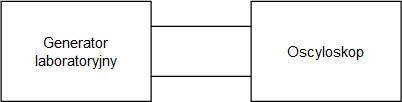
\includegraphics{schemat}
        \caption{logo}
        \end{figure}

    \begin{figure}[H]
        \begin{center}
        \begin{tikzpicture}[>=latex,every node/.style={draw,rectangle,minimum width={3em},node distance=6em}]
        \node (a) {1};
        \node [below left of=a] (b) {2}; 
        \node [below left of=b] (d) {4}; 
        \node [below right of=a] (c) {3}; 
        \node [below right of=c] (e) {5}; 
        \draw [->] (b) -- (a);
        \draw [->] (c) -- (a);
        \draw [->] (c) -- (b);
        \draw [<->] (b) -- (d);
        \draw [<->] (c) -- (e);
        \end{tikzpicture}
        \caption{This is a figure}
        \end{center}
        \end{figure}



\subsection{wzory}
%\alpha \beta \gamma \rho \sigma \delta \epsilon \times \otimes \oplus \cup \cap
\(\int \frac{1}{x^2_0}
\)
%\clearpage
\section{Pomiary i obliczenia}
\subsection{Pomiary}
\begin{table}[H]
\centering
\resizebox{\textwidth}{!}{%
\begin{tabular}{|c|c|c|c|c|c|c|c|c|c|c|}
\hline
\begin{tabular}[c]{@{}c@{}}
\diagbox[height=3em,width=12em]{ Nr. Pomiaru}{Wartość napięcia}\end{tabular} 
& 1 & 2 & 3 & 4 & 5 & 6 & 7 & 8 & 9 & 10 \\ \hline
1V  & 1.4 & 1.5 & 1.6 & 1.7 & 1.8 & 1.9 & 2   & 2.1 & 2.2 & 2.3 \\ \hline
3V  & 1.7 & 1.8 & 1.9 & 2   & 2.1 & 2.2 & 2.3 & 2.4 & 2.5 & 2.6 \\ \hline
5V  & 2.8 & 2.9 & 3   & 3.1 & 3.2 & 3.3 & 3.4 & 3.5 & 3.6 & 3.7 \\ \hline
10V & 3   & 3.1 & 3.2 & 3.3 & 3.4 & 3.5 & 3.6 & 3.7 & 3.8 & 3.9 \\ \hline
12V & 3.5 & 3.6 & 3.7 & 3.8 & 3.9 & 4   & 4.1 & 4.2 & 4.3 & 4.4 \\ \hline
\end{tabular}%
}
\end{table}

\subsection{Obliczenia}
\section{Wyniki i Wnioski}
\end{document}
